\chapter{Μεθοδολογία}\label{ch:methodology}
\section{Επισκόπηση του συστήματος}\label{sec:overview}
\subsection{Στόχος της υλοποίησης}\label{ssec:goal}
Η παρούσα εργασία επικεντρώνεται στη δημιουργία ενός federated μοντέλου για την επίλυση του προβλήματος της σύστασης κανόνων. Αξιοποιεί τα δεδομένα που παρείχε η Wyze στον διαγωνισμό της, σε μορφή δύο ζευγών αρχείων CSV: το πρώτο περιγράφει τις συσκευές κάθε χρήστη και το δεύτερο τους κανόνες μεταξύ τους. Η φύση και οι ιδιαιτερότητες των δεδομένων αναλύονται εκτενέστερα στην \autoref{sec:exp-data}. Στόχος της υλοποίησης είναι να καταδείξει την αντιστάθμιση μεταξύ ιδιωτικότητας και επίδοσης, με συμπληρωματικό στόχο μια ανταγωνιστική επίδοση σε σχέση με τη δεύτερη θέση του διαγωνισμού.

\subsection{Ανάπτυξη των μοντέλων}\label{ssec:versions}
Η ανάπτυξη της τελικής υλοποίησης ακολούθησε μια επαναληπτική διαδικασία, η οποία διακρίνεται σε τρεις εκδόσεις:
\begin{itemize}
    \item Η πρώτη έκδοση (v1) υλοποιεί έναν βασικό federated αλγόριθμο, βασισμένο στη δημοσίευση της Wyze, χωρίς τα edge-type embeddings του μοντέλου της δεύτερης θέσης. Στόχος της είναι η επιβεβαίωση της λειτουργικότητας του federation και η εξαγωγή baseline αποτελεσμάτων. Συμπληρωματικά, αναπτύχθηκε μια βοηθητική συνάρτηση προεπεξεργασίας, ύστερα από τον εντοπισμό ελλείψεων και ασυνεπειών στο σύνολο δεδομένων της Wyze (\autoref{ssec:v1-preprocessing}).
    \item Η δεύτερη έκδοση (v2) εισάγει edge-type embeddings, ακολουθώντας πιστά την υλοποίηση της δεύτερης θέσης. Όπως διασαφηνίζεται στην \autoref{sec:v2}, πρόκειται για «pseudo-embeddings», καθώς το ίδιο το μοντέλο δεν υποστηρίζει πραγματικά embeddings. Στόχος της είναι η άμεση, «ένα προς ένα» σύγκριση δύο πανομοιότυπων μοντέλων, με μοναδική διαφοροποίηση την federated ενορχήστρωση.
    \item Η τρίτη έκδοση (v3) στηρίζεται στις βελτιώσεις της προηγούμενης και τις επαυξάνει, εισάγοντας πραγματικά edge-type embeddings και έναν βελτιωμένο relational decoder, καθώς και μια εναλλακτική συνάρτηση σφάλματος. (\autoref{sec:v3}). Στόχος της είναι η βελτιστοποίηση του μοντέλου και η αναζήτηση αποδοτικότερης λύσης στο πρόβλημα. Συνοδεύεται από ablation studies υπερπαραμέτρων, με σκοπό τον εντοπισμό των βέλτιστων συνθηκών εκπαίδευσης.
\end{itemize}

\subsection{Δομή του κώδικα}\label{ssec:codebase}
Για την εκπαίδευση όλων των μοντέλων σε federated περιβάλλον χρησιμοποιήθηκε το Flower \cite{beutel_flower_2020, flower_software}, μια βιβλιοθήκη της Python για την προσομοίωση και την ενορχήστρωση federated υλοποιήσεων. Περισσότερες πληροφορίες για τη βιβλιοθήκη, καθώς και για τα υπόλοιπα εργαλεία των προσομοιώσεων, παρατίθενται στην \autoref{sec:exp-tools}. Με στόχο να εναρμονιστεί με τη δομή λειτουργίας του framework, ο κώδικας της παρούσας εργασίας οργανώνεται σε επτά διακριτά αρχεία:
\begin{itemize}
    \item Στο \ident{dataset.py} βρίσκονται οι βοηθητικές συναρτήσεις για την αρχικοποίηση του συνόλου δεδομένων, το φιλτράρισμα και τον καθαρισμό του, τη δημιουργία του λεξιλογίου συσκευών και κανόνων, και τη μετατροπή του σε μορφή γράφων.
    \item Στο \ident{server_app.py} ορίζεται ο server, μαζί με τις συναρτήσεις aggregation και κεντρικής αξιολόγησης.
    \item Στο \ident{client_app.py} ορίζονται οι clients, μαζί με τη συνάρτηση fit για την τοπική εκπαίδευση και βοηθητικές συναρτήσεις για τη λήψη και αποστολή των βαρών από και προς τον server.
    \item Στο \ident{model.py} ορίζονται τα διαφορετικά μοντέλα που εκπαιδεύουν οι clients.
    \item Στο \ident{task.py} περιέχονται οι συναρτήσεις για την εφαρμογή leave-one-out και negative sampling, καθώς και η λογική ενορχήστρωσης της τοπικής εκπαίδευσης.
    \item Στο \ident{pyproject.toml} ορίζονται όλες οι υπερπαράμετροι εκπαίδευσης (αριθμός clients, local epochs, στρατηγική συνάθροισης, optimizer κ.ά.).
    \item Στο \ident{results_logger.py} βρίσκονται βοηθητικές συναρτήσεις για την καταγραφή των μετρικών ενός run και την δημιουργία checkpoints με τα καλύτερα μοντέλα.
\end{itemize}
Και οι τρεις εκδόσεις ακολουθούν αυτή τη δομή. Τα πειράματα προκύπτουν εκτελώντας το ίδιο πρόγραμμα με διαφορετικές παραμέτρους.
Ο πλήρης κώδικας της εργασίας είναι διαθέσιμος στο \cite{politis_code_2026}.

\section{Πρώτη έκδοση (v1)}\label{sec:v1}
\subsection{Προεπεξεργασία δεδομένων}\label{ssec:v1-preprocessing}
Τα δεδομένα του διαγωνισμού προέρχονται από ένα ιδιωτικό σύνολο της Wyze, το οποίο η εταιρεία ανωνυμοποίησε \cite{noauthor_wyzelabsrulerecommendation_nodate} και διέθεσε σε δύο ζεύγη αρχείων (train και test), που αφορούν τις συσκευές των χρηστών (\ident{train_device.csv}, \ident{test_device.csv}) και τους μεταξύ τους κανόνες (\ident{train_rule.csv}, \ident{test_rule.csv}) αποσπάσματα των οποίων παρουσιάζονται στους Πίνακες \ref{tab:devices} και \ref{tab:rules}:
\begin{itemize}
    \item \ident{train_device.csv}: Περιέχει τις συσκευές όλων των χρηστών. Αποτελείται από τρεις στήλες: η πρώτη περιέχει ένα μοναδικό αναγνωριστικό (ID) για κάθε χρήστη (π.χ. 115535), η δεύτερη ένα μοναδικό αναγνωριστικό για κάθε συσκευή κάθε χρήστη (π.χ. 942835), και η τρίτη το μοντέλο της συσκευής (π.χ. Light). Έτσι, μια γραμμή διαβάζεται ως «ο χρήστης 115535 κατέχει τη συσκευή 942835, η οποία είναι λαμπτήρας». Κάθε συσκευή έχει το δικό της αναγνωριστικό ακόμη και αν είναι ίδιου τύπου με άλλες: αν ένας χρήστης διαθέτει τρεις πανομοιότυπες κάμερες, η καθεμία έχει ξεχωριστό ID αλλά κοινό μοντέλο «Camera»· αντίστοιχα, αν δύο χρήστες διαθέτουν το ίδιο μοντέλο, ο καθένας έχει το δικό του ID.
    \item \ident{train_rule.csv}: Περιέχει τους κανόνες που έχει ορίσει κάθε χρήστης ανάμεσα στις συσκευές του. Αποτελείται από δέκα στήλες. Η πρώτη περιέχει το μοναδικό ID του χρήστη (π.χ. 257281), το οποίο αντιστοιχίζεται ένα προς ένα με εκείνα του \ident{train_device.csv}. Η δεύτερη και η τρίτη περιέχουν το μοντέλο (π.χ. «ContactSensor») και το ID (π.χ. 559037) της συσκευής που πυροδοτεί τον κανόνα (trigger device). Η τέταρτη και η πέμπτη περιέχουν την κατάσταση (state) στην οποία πρέπει να βρίσκεται η συσκευή (π.χ. «Detects a person») και ένα μοναδικό ID για την κατάσταση αυτή (π.χ. 6). Η έκτη και η έβδομη περιέχουν τη δράση (action) που ενεργοποιείται, μαζί με το ID της, και η όγδοη και ένατη το μοντέλο και το ID της συσκευής που ενεργοποιείται (action device). Η τελευταία στήλη συγχωνεύει τα προηγούμενα IDs. Για παράδειγμα, η πρώτη γραμμή του Πίνακα \ref{tab:rules} διαβάζεται ως: «ο χρήστης 289923 έχει ορίσει έναν κανόνα σύμφωνα με τον οποίο, όταν η συσκευή 1507149 (κάμερα) εντοπίσει ένα κατοικίδιο (ID=7), τότε η συσκευή 1492326 (κάμερα) τίθεται σε λειτουργία (ID=41)».
\end{itemize}

Τα αρχεία \ident{test_device.csv} και \ident{test_rule.csv} έχουν ακριβώς την ίδια δομή με τα παραπάνω, αλλά αφορούν το σύνολο δεδομένων που χρησιμοποιείται για την αξιολόγηση του μοντέλου.

\begin{table}[htbp]
  \centering
  \begin{tabular}{r r l}
    \toprule
    \ident{user_id} & \ident{device_id} & \ident{device_model} \\
    \midrule
    115535 & 107235  & Lock          \\
    115535 & 511842  & MotionSensor  \\
    115535 & 1793633 & ContactSensor \\
    115535 & 463524  & ContactSensor \\
    115535 & 572702  & Light         \\
    115535 & 562426  & MotionSensor  \\
    115535 & 120593  & Camera        \\
    115535 & 1340294 & Camera        \\
    115535 & 942835  & Light         \\
    115535 & 1108491 & Camera        \\
    ...    & ...     & ...           \\
    289923 & 1507149 & Camera        \\
    289923 & 1492326 & Camera        \\
    \bottomrule
  \end{tabular}
  \caption[Απόσπασμα του συνόλου δεδομένων \ident{train_device.csv}]{Απόσπασμα του \ident{train_device.csv}: οι δέκα συσκευές του χρήστη 115535 και οι δύο του χρήστη 289923. Συσκευές ίδιου μοντέλου (δύο \emph{Light}, πέντε \emph{Camera}, δύο \emph{MotionSensor}, δύο \emph{ContactSensor}) έχουν διαφορετικά αναγνωριστικά.}
  \label{tab:devices}
\end{table}

\begin{table}[htbp]
  \centering
  \footnotesize
  \setlength{\tabcolsep}{4pt}
  \begin{tabular}{r l r l r l r l r}
    \toprule
    & \multicolumn{4}{c}{\textbf{Trigger}} & \multicolumn{4}{c}{\textbf{Action}} \\
    \cmidrule(lr){2-5}\cmidrule(lr){6-9}
    \ident{user} & \ident{device} & \ident{id} & \ident{state} & \ident{id} & \ident{action} & \ident{id} & \ident{device} & \ident{id} \\
    \midrule
    289923 & Camera        & 1507149 & Detects a pet    & 7  & Turn on the camera   & 41 & Camera & 1492326 \\
    289923 & Camera        & 1507149 & Detects a pet    & 7  & Unmute Notifications & 45 & Cloud  & 1797174 \\
    257281 & ContactSensor & 1769589 & Opens            & 25 & Turn on              & 30 & Light  & 265706  \\
    257281 & MotionSensor  & 1521508 & Detects motion   & 9  & Turn on              & 30 & Light  & 399694  \\
    257281 & Camera        & 275358  & Detects a person & 6  & Turn on for          & 34 & Light  & 371957  \\
    257281 & Switch        & 1752653 & Double Press     & 12 & Turn on              & 30 & Plug   & 1327057 \\
    \bottomrule
  \end{tabular}
  \caption[Απόσπασμα του συνόλου δεδομένων \ident{train_rules.csv}]{Απόσπασμα του \ident{train_rule.csv} (η τελευταία στήλη \ident{rule}, που συνενώνει τα τέσσερα IDs, παραλείπεται). Η πρώτη γραμμή αντιστοιχεί στο παράδειγμα του κειμένου. H δεύτερη δείχνει τη νοητή συσκευή \emph{Cloud}, η οποία εμφανίζεται μόνο στους κανόνες. Οι κανόνες του χρήστη 289923 αντιστοιχίζονται στις συσκευές που εμφανίζονται στον Πίνακα \ref{tab:devices}.}
  \label{tab:rules}
\end{table}

\begin{figure}[htbp]
  \centering
  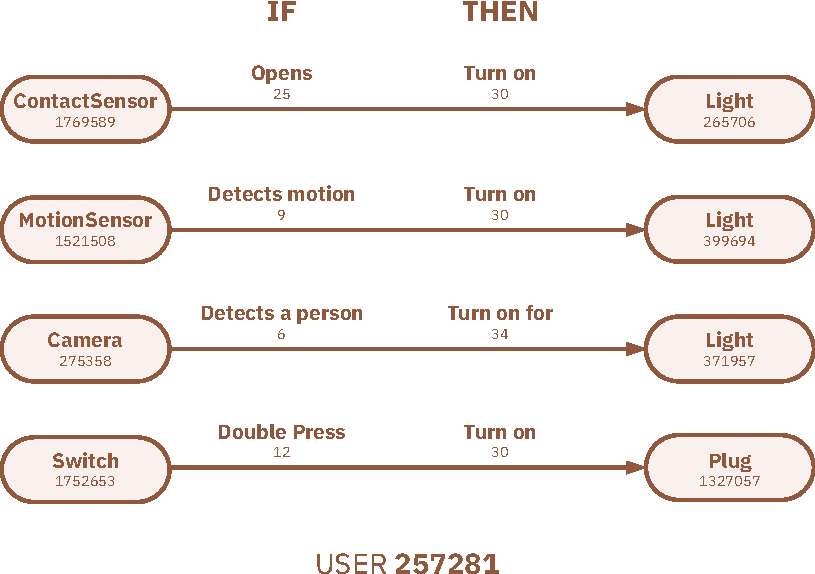
\includegraphics[width=0.95\linewidth]{./assets/images/user-graph}
  \caption[Παράδειγμα γράφου χρήστη]{Παράδειγμα του γράφου του χρήστη 257281. Ο χρήστης κατέχει 8 συσκευές και 4 κανόνες μεταξύ τους. Στις τελευταίες 4 γραμμές του Πίν. \ref{tab:rules} φαίνονται οι εγγραφές του.}
  \label{fig:user-graph}
\end{figure}

Με στόχο την επιβεβαίωση της ορθότητας και της καθαρότητας του συνόλου δεδομένων, πραγματοποιήθηκε ανάλυσή του, η οποία απάντησε σε ερωτήματα όπως «πόσοι διαφορετικοί χρήστες υπάρχουν;», «πόσες συσκευές κατέχει κατά μέσο όρο κάθε χρήστης;» και «ποιος κανόνας εμφανίζεται συχνότερα;». Κυρίως όμως, οδήγησε στη διαπίστωση ότι αρκετές συσκευές συμμετέχουν σε κάποιον κανόνα στο \ident{train_rule.csv}, ενώ απουσιάζουν από τη λίστα συσκευών του αντίστοιχου χρήστη στο \ident{train_device.csv}, μένοντας πρακτικά αναξιοποίητες, ή «φαντάσματα» (ghosts).

Η υλοποίηση της δεύτερης θέσης απορρίπτει αυτές τις συσκευές, αποκλείοντας σημαντικό όγκο δεδομένων από την εκπαίδευση. Ύστερα από εκτενέστερη μελέτη, διαπιστώθηκε ότι πρόκειται για έγκυρα δεδομένα που ακολουθούν τις ίδιες κατανομές με τις υπόλοιπες συσκευές και σχηματίζουν εξίσου έγκυρους κανόνες, και επομένως μπορούν να προσφέρουν χρήσιμη πληροφορία στην εκπαίδευση. Για τον λόγο αυτό, εισήχθη κατά το preprocessing η βοηθητική συνάρτηση \ident{resurrect_ghosts()}, η οποία προσθέτει τις συσκευές «φαντάσματα» στη λίστα συσκευών κάθε χρήστη. Σε πειραματικό επίπεδο, η συνάρτηση μπορεί να απενεργοποιηθεί μέσω του αντίστοιχου flag (\autoref{ssec:orchestration}).

Πέρα από αυτή τη διαφοροποίηση, η προετοιμασία των δεδομένων δεν διαφέρει ουσιαστικά από εκείνη της δεύτερης θέσης: τα αρχεία φορτώνονται από τοπικό φάκελο ή απευθείας από τη σελίδα του διαγωνισμού στο HuggingFace, παράγεται το λεξιλόγιο όλων των μοναδικών τύπων συσκευών και κανόνων, φιλτράρονται οι κανόνες που εμφανίζονται λιγότερες από έναν καθορισμένο αριθμό φορών, ώστε το μοντέλο να εκπαιδευτεί σε συχνά εμφανιζόμενα μοτίβα, αντιστοιχίζονται οι συσκευές «φαντάσματα» και, τέλος, τα δεδομένα μετατρέπονται σε γράφους (PyG tensors).

\subsection{Μοντέλα μηχανικής μάθησης}\label{ssec:v1-models}
Τα μοντέλα της πρώτης έκδοσης ταυτίζονται με εκείνα της υλοποίησης της Wyze. Όπως αναφέρθηκε στην \autoref{sec:wyze-baseline}, για το node embedding χρησιμοποιείται ένα GraphSAGE \cite{hamilton_inductive_2017} με δύο επίπεδα SAGEConv, mean aggregation και ενεργοποίηση ReLU μετά το πρώτο επίπεδο, ενώ για το link prediction ένα MLP δύο επιπέδων.

\begin{figure}[htbp]
  \centering
  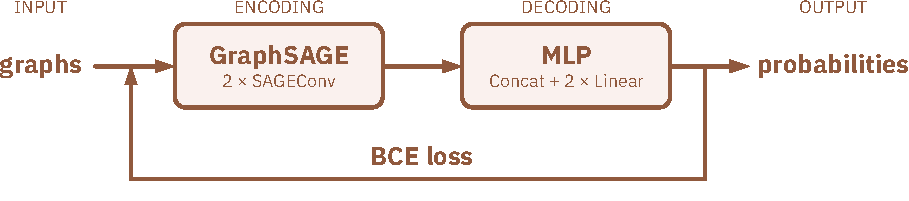
\includegraphics[width=0.95\linewidth]{./assets/images/v1-pipeline}
  \caption[Pipeline πρώτης έκδοσης]{Pipeline πρώτης έκδοσης: Το encoding των γράφων γίνεται μέσω του GraphSAGE, ενώ το decoding μέσω ενός MLP.}
  \label{fig:v1-pipeline}
\end{figure}

\subsection{Ενορχήστρωση}\label{ssec:orchestration}
Όλες οι παράμετροι της πειραματικής διαδικασίας ρυθμίζονται κατά την κλήση της κύριας συνάρτησης της προσομοίωσης: ο ελάχιστος επιτρεπόμενος αριθμός εμφανίσεων ανά κανόνα, η ενεργοποίηση ή μη της επαναφοράς «φαντασμάτων», ο ρυθμός μάθησης, ο αριθμός των local epochs, η στρατηγική συνάθροισης, ο τοπικός optimizer κ.ά. Με την κλήση της συνάρτησης αρχικοποιείται το περιβάλλον του Flower, το οποίο με τη σειρά του αρχικοποιεί τον server και τους clients, φορτώνει το σύνολο δεδομένων στη μνήμη και ενορχηστρώνει την εκπαίδευση. Σε κάθε γύρο υπολογίζονται οι μετρικές, οι οποίες συνοψίζονται στο τέλος της εκπαίδευσης.

\section{Δεύτερη έκδοση (v2)}\label{sec:v2}
Η δεύτερη έκδοση διαφοροποιείται από την πρώτη μόνο ως προς το μοντέλο που εκπαιδεύεται. Η διαχείριση των δεδομένων, οι υπερπαράμετροι και η ενορχήστρωση της εκπαίδευσης παραμένουν ίδιες με πριν. Η υλοποίηση μιμείται εκείνη της δεύτερης θέσης, ενσωματώνοντας edge-type embeddings στους κόμβους των γράφων πριν από την είσοδό τους στο GraphSAGE. Όπως αναλύθηκε στις Ενότητες \ref{ssec:weaknesses} και \ref{sec:second-place}, η κωδικοποίηση του τύπου κάθε κανόνα εμπλουτίζει σημαντικά την πληροφορία που διαθέτει το δίκτυο και βελτιώνει τις επιδόσεις του μοντέλου. Για τον λόγο αυτό, η διαφοροποίηση αυτή μελετάται πειραματικά.

Συγκεκριμένα, πριν οι γράφοι φορτωθούν στο GraphSAGE, εισάγονται δύο πίνακες embeddings: ένας για την κατάσταση που πυροδοτεί τον κανόνα (trigger state) και ένας για τη δράση που ενεργοποιείται (action). Για κάθε ακμή του γράφου, το trigger embedding συνενώνεται μέσω concatenation με τον κόμβο trigger device και το action embedding με τον κόμβο του action device.

Η προσέγγιση αυτή χαρακτηρίζεται ως pseudo-embeddings» γιατί η πληροφορία του τύπου των κανόνων δεν αξιοποιείται εγγενώς κατά το message passing. Το GraphSAGE δεν έχει την αρχιτεκτονική δυνατότητα να περάσει το vector του τύπου κάθε ακμής ξεχωριστά μέσα από τα layers του. Η δεύτερη έκδοση προσπαθεί να προσεγγίσει αυτή την λειτουργικότητα μέσω του aggregation και concatenation αυτής της πληροφορίας στους ίδιους τους κόμβους πριν από το GNN. Εμπλουτίζει δηλαδή το feature vector κάθε κόμβου (που καθορίζει τι είδους συσκευή είναι) με το vector του τύπου των συνδέσεών του (που καθορίζει πώς συνδέεται με άλλες συσκευές). Το ίδιο το GNN εξακολουθεί να αντιμετωπίζει τις ακμές ως απλές συνδέσεις χωρίς τύπο, έχοντας όμως μία εικόνα για το ποιος θα μπορούσε να είναι αυτός μέσω των εμπλουτισμένων feature vectors των κόμβων. Πρόκειται δηλαδή για μια προσέγγιση των πραγματικών edge embeddings, τα οποία υλοποιούνται στην τρίτη έκδοση (\autoref{sec:v3}). Το \autoref{fig:pseudo-embeddings} αναδεικνύει αυτή την διαφοροποίηση.

\begin{figure}[htbp]
  \centering
  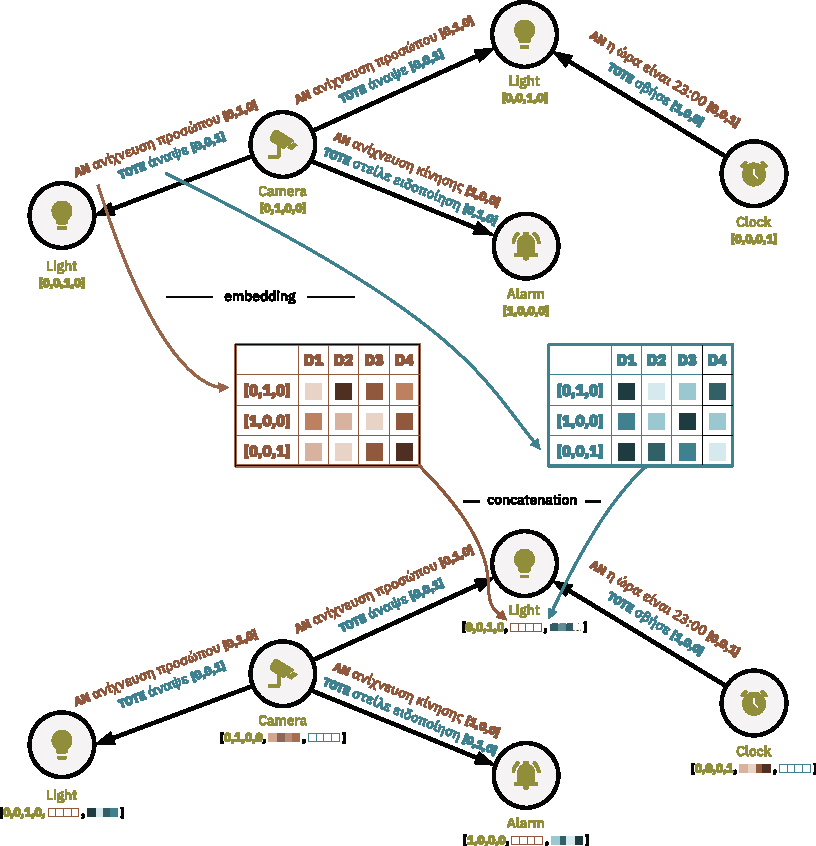
\includegraphics[width=\linewidth]{./assets/images/pseudo-embeddings}
  \caption[Pseudo-embeddings της v2]{Pseudo-embeddings: οι αναπαραστάσεις των τύπων ακμών (πάνω), π.χ. [0,1,0] για το trigger «ανίχνευση προσώπου» και [0,0,1] για το action «άναψε», μετατρέπονται σε δύο embeddings τεσσάρων διαστάσεων (μέση) και γίνονται concatenate (κάτω) με τους τύπους των συσκευών. Στο παράδειγμα όλες οι συσκευές είναι είτε sources είτε destinations, αλλά μία συσκευή μπορεί να είναι και τα δύο.}
  \label{fig:pseudo-embeddings}
\end{figure}

\begin{figure}[htbp]
  \centering
  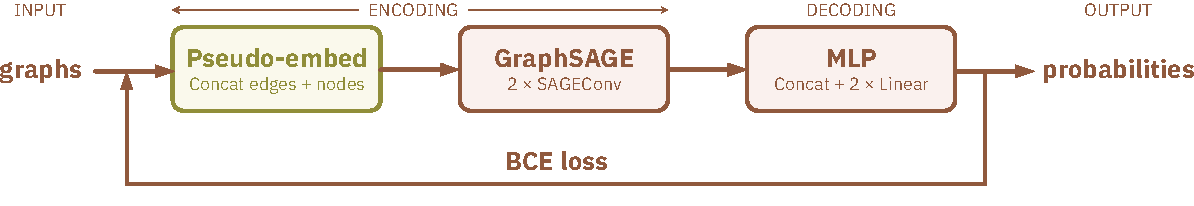
\includegraphics[width=\linewidth]{./assets/images/v2-pipeline}
  \caption[Pipeline δεύτερης έκδοσης]{Pipeline δεύτερης έκδοσης: Πριν την είσοδο στο GraphSAGE, οι τύποι των ακμών ενσωματώνονται στους κόμβους μέσω των pseudo-embeddings.}
  \label{fig:v2-pipeline}
\end{figure}

\section{Τρίτη έκδοση (v3)}\label{sec:v3}
Η τρίτη έκδοση (v3) αποτελεί μια απόπειρα βελτιστοποίησης του συστήματος σε όλους τους τομείς του. Εξετάζει διαφορετικές αρχιτεκτονικές τόσο στην κωδικοποίηση της δομής των γράφων (CompGCN \cite{vashishth_composition_2020} αντί για GraphSAGE) όσο και στην αποκωδικοποίησή της και την πρόβλεψη ακμών (ComplEx \cite{trouillon_complex_2016} αντί για MLP). Επιπλέον, υλοποιεί μία διαφορετική συνάρτηση σφάλματος, προσαρμοσμένη στο πρόβλημα προς επίλυση \cite{oord_representation_2018}.

\subsection{CompGCN encoder}
Όπως αναφέρθηκε στην \autoref{sec:v2}, η υλοποίηση της δεύτερης έκδοσης αξιοποιεί το GraphSAGE για τα embeddings των συσκευών των χρηστών (κόμβων), το οποίο ωστόσο δεν έχει την δυνατότητα να αναπαραστήσει τα εξίσου σημαντικά embeddings των κανόνων (ακμών). Τα embeddings αυτά προσεγγίστηκαν μέσω του aggregation και του concatenation των τύπων των ακμών στους κόμβους πριν το encoding του GraphSAGE. Η τρίτη έκδοση της υλοποίησης αλλάζει την αρχιτεκτονική του encoding, αξιοποιώντας πλέον πραγματικά τους τύπους των κανόνων, μέσω του CompGCN (\autoref{fig:compgcn}).

Το CompGCN είναι ένα δίκτυο GNN εξειδικευμένο στην αναπαράσταση multi-relational γράφων \cite{nickel_review_2016}, δηλαδή γράφων που υποστηρίζουν πολλαπλούς τύπους ακμών, όπως αυτό του \autoref{fig:multi-relational}. Η βασική ιδέα είναι ότι κατά την διαδικασία του message passing από έναν γείτονα, δεν μεταφέρεται μόνο το feature vector του, αλλά η σύνθεσή του με τον τύπο της ακμής που τον συνδέει με τον υπό ανάλυση κόμβο (στην παρούσα εργασία πολλαπλασιασμός κατά στοιχείο) \cite{vashishth_composition_2020}. Έτσι, το δίκτυο αφομοιώνει πραγματικά μέσα στην αρχιτεκτονική του τους τύπους των κανόνων που συνδέουν τις συσκευές, και όχι τεχνητά μέσω ενός απλού pre-processing σταδίου. Επιπλέον, η αρχιτεκτονική του CompGCN αποθηκεύει εγγενώς τις αναπαραστάσεις των τύπων των κανόνων σε κάθε layer της, γεγονός που διευκολύνει το επόμενο στάδιο της διαδικασίας: το decoding.

\begin{figure}[htbp]
  \centering
  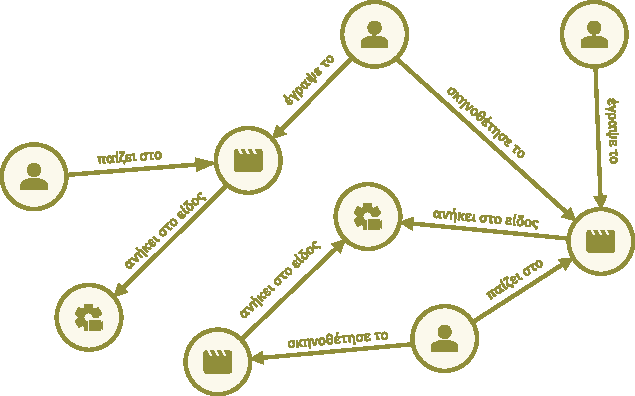
\includegraphics[width=0.85\linewidth]{./assets/images/multi-relational}
  \caption[Multi-relational γράφος]{Παράδειγμα multi-relational γράφου: οι κόμβοι συνδέονται με 4 διαφορετικούς τύπους ακμών («έγραψε το», «σκηνοθέτησε το», «παίζει στο», και «ανήκει στο είδος»).}
  \label{fig:multi-relational}
\end{figure}

\begin{figure}[htbp]
  \centering
  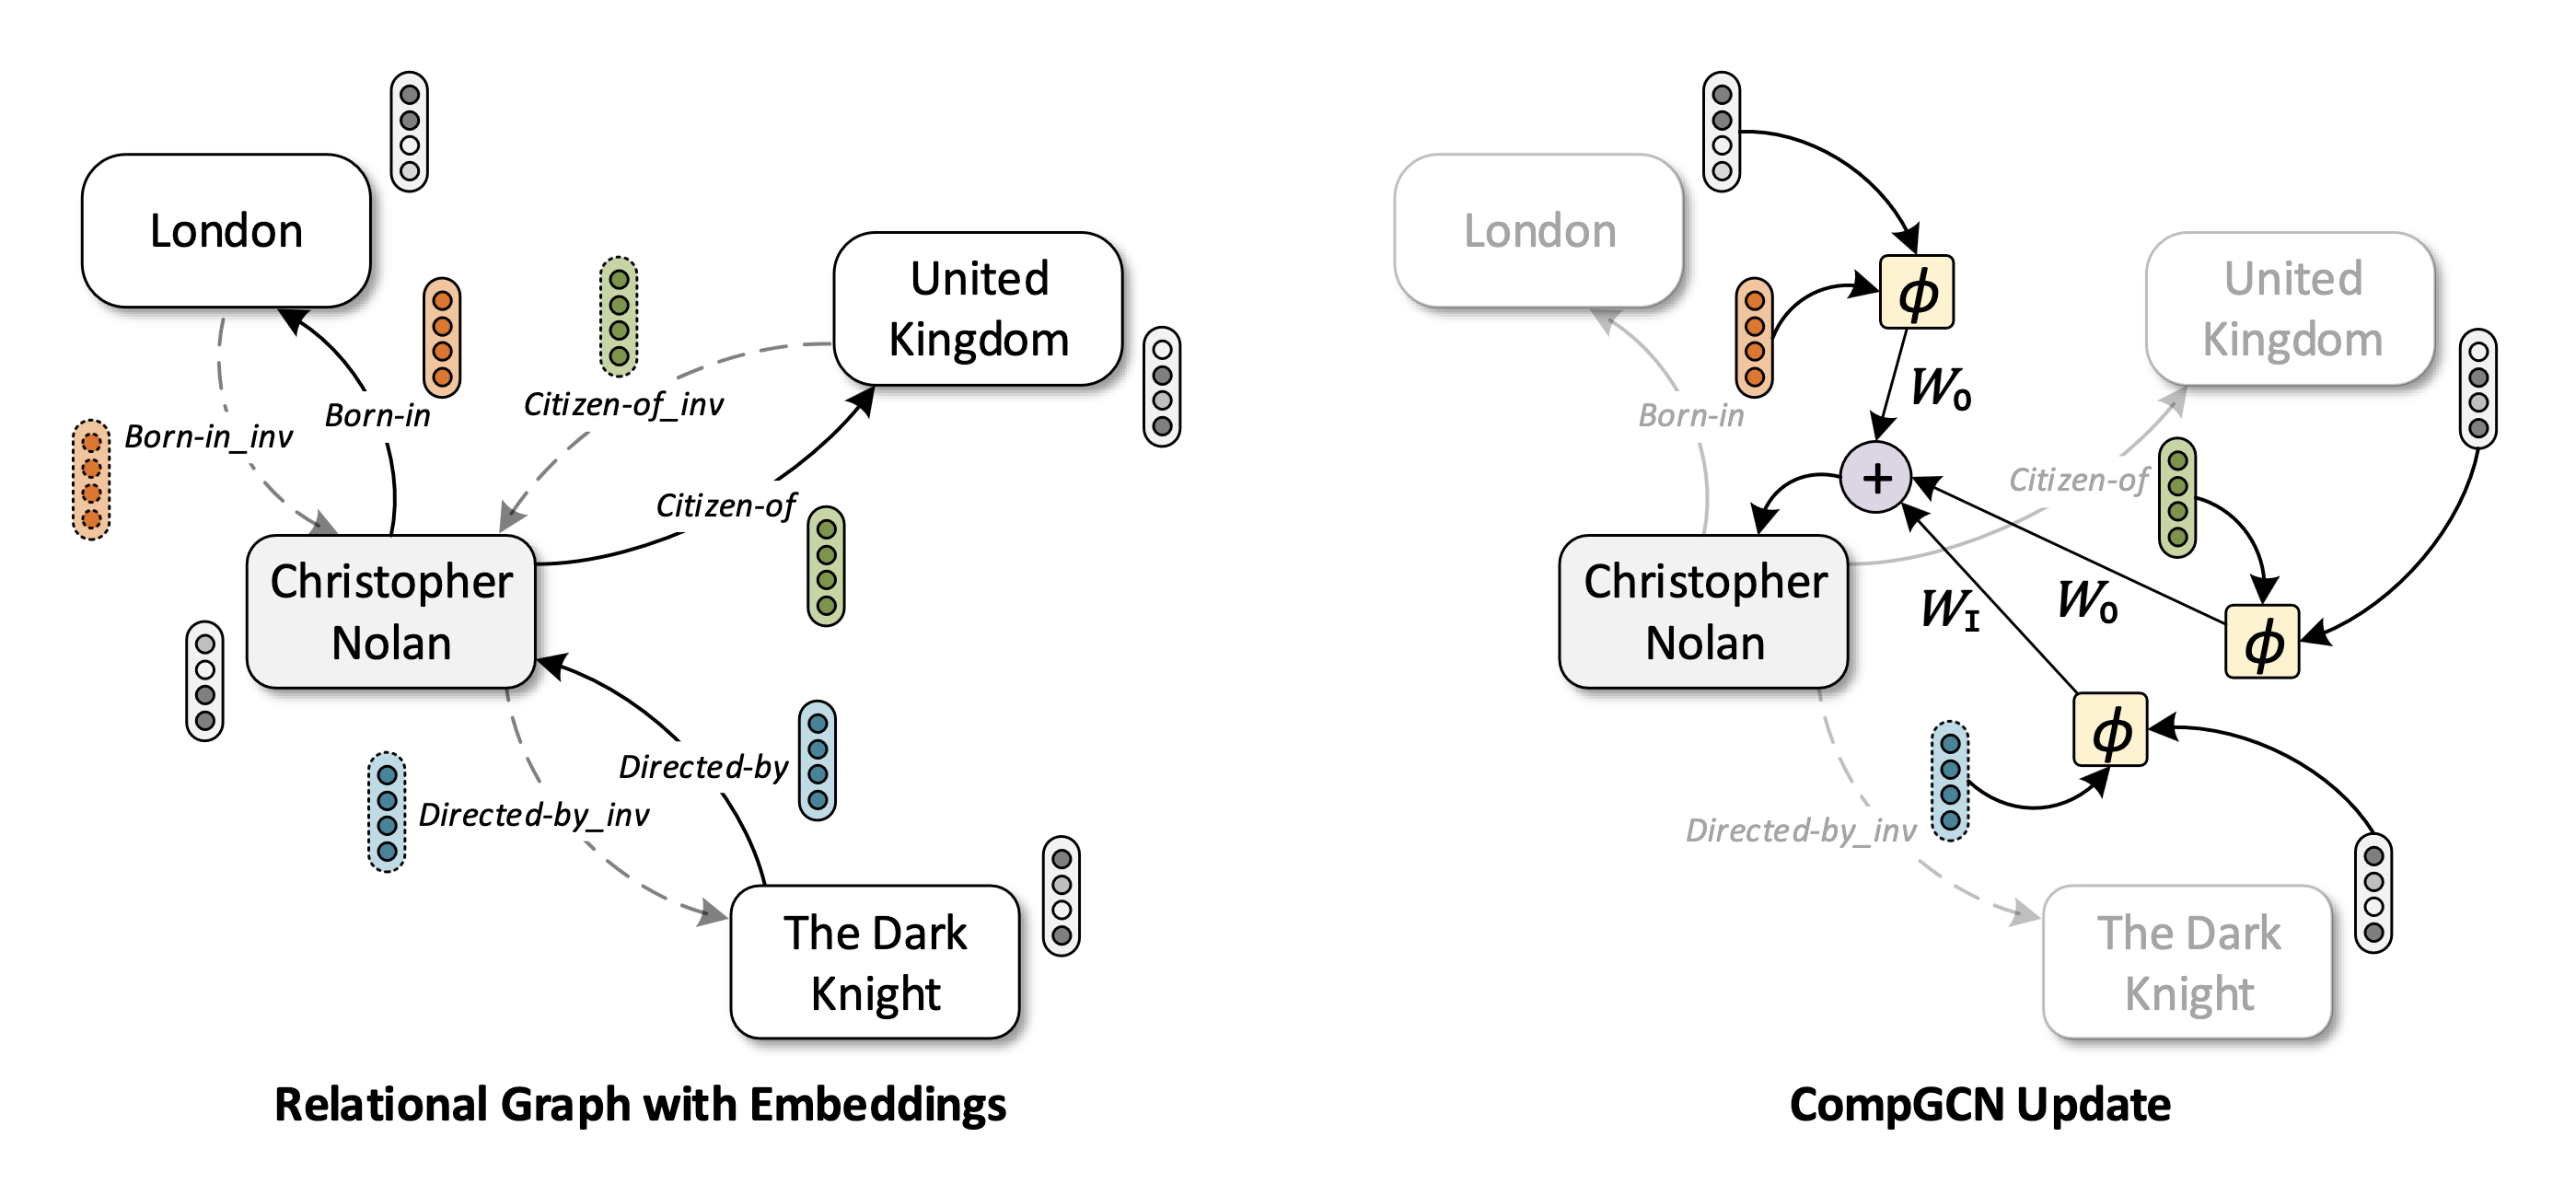
\includegraphics[width=\linewidth]{./assets/images/compgcn}
  \caption[Αρχιτεκτονική CompGCN]{Η αρχιτεκτονική του CompGCN: κάθε μήνυμα συνθέτει την αναπαράσταση του γείτονα με εκείνη του τύπου της ακμής που τους συνδέει μέσω της συνάρτησης σύνθεσης $φ$ \cite{vashishth_composition_2020}.}
  \label{fig:compgcn}
\end{figure}

\subsection{ComplEx decoder}\label{ssec:complex}
Μέχρι στιγμής, το δεύτερο στάδιο του μοντέλου, αυτό της πρόβλεψης μιας νέας ακμής, αποτελούνταν από ένα απλό MLP που προσπαθούσε να μάθει μία γενικευμένη συνάρτηση ελαχιστοποίησης του σφάλματος πρόβλεψης (\autoref{sec:v2}). Στην τρίτη έκδοση αντικαθίσταται από το ComplEx, έναν εξειδικευμένο relational decoder, ο οποίος βαθμολογεί απευθείας κάθε τριπλέτα συσκευή-κανόνας-συσκευή μέσω ενός τριγραμμικού γινομένου σε μιγαδικό διανυσματικό χώρο (\autoref{fig:complex}).

Η ειδοποιός διαφορά σε σχέση με το MLP είναι ότι το ComplEx ενσωματώνει τους κανόνες στο ίδιο το score μέσω του embedding του, αξιολογώντας άμεσα κάθε τριπλέτα, ενώ το MLP δεν μπορεί παρά μόνο να τους κάνει concatenate στην γενικευμένη softmax συνάρτησή του.

Η επιλογή ενός μιγαδικού χώρου ενέχει το σημαντικό πλεονέκτημα της δυνατότητας αναπαράστασης ασύμμετρων σχέσεων: ο κανόνας «η συσκευή Α πυροδοτεί την Β» είναι προφανώς εννοιολογικά διαφορετικός από την αντίστροφό του, και το ComplEx διαχωρίζει αυτά τα δύο σενάρια, σε αντίθεση με άλλους decoders όπως ο DistMult \cite{yang_embedding_2015}, επιτρέποντας έτσι μία στιβαρή αξιολόγηση \cite{trouillon_complex_2016}.

\begin{figure}[ht]
  \centering
  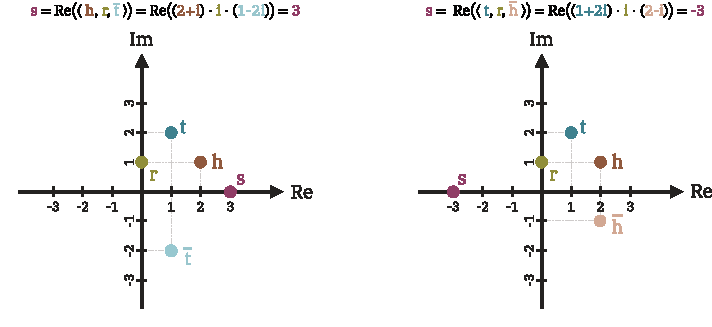
\includegraphics[width=\linewidth]{./assets/images/complex}
  \caption[Αρχιτεκτονική ComplEx]{Το ComplEx decoder βαθμολογεί μια τριπλέτα $(h,r,t)$, όπου h (head) = trigger device, r (relation) = rule, t (tail) = action device, με το τριγραμμικό γινόμενο $\mathrm{Re}(\langle h,r,\bar t\rangle)$ στο μιγαδικό επίπεδο, όπου $\bar t$ το συζυγές του tail. Επειδή η εναλλαγή των ρόλων head/tail μετακινεί την συζυγία, το score που ανατίθεται στον κανόνα «h→t» $s=\mathrm{Re}(\langle h,r,\bar t\rangle)$ (αριστερά) είναι διαφορετικό από αυτό που ανατίθεται στον κανόνα «t→h» $s=\mathrm{Re}(\langle t,r,\bar h\rangle)$. Αυτή η ιδιότητα επιτρέπει την αναπαράσταση κατευθυνόμενων κανόνων.}
  \label{fig:complex}
\end{figure}

\subsection{InfoNCE loss και hard negative sampling}\label{ssec:infonce}
Τέλος, η τρίτη έκδοση εισάγει μία νέα συνάρτηση σφάλματος κατά την διαδικασία του training. Η BCE (\autoref{sec:v2}) αντικαθίσταται από την InfoNCE (\autoref{fig:infonce}), που στόχο έχει να αναγνωρίσει την επιθυμητή (θετική) ακμή ανάμεσα σε $k$ αρνητικές, μελετώντας την διαφοροποίηση στην στοχαστική πληροφορία που περιέχουν ως τυχαίες μεταβλητές (συγκεκριμένα, αποτελεί μια συνάρτηση προσέγγισης του Mutual Information \cite{oord_representation_2018, cover_elements_2006} αυτών των τυχαίων μεταβλητών). Η InfoNCE αποτελεί ειδική περίπτωση της CCE (Categorical Cross-Entropy loss), η οποία παρουσιάζει στενότερο θεωρητικό κάτω φράγμα MRR από την BCE \cite{diteodoro_theoretical_2024} και έτσι μπορεί δυνητικά να αποδώσει καλύτερα αποτελέσματα με την κατάλληλη παραμετροποίηση. Στην παρούσα εργασία, κατόπιν ablation της παραμέτρου $k$ (βλ. \autoref{ssec:exp-ablations}), διαπιστώθηκε ότι η τιμή $k=64$ για τα negative samples αποδίδει ικανοποιητικά αποτελέσματα.

Για να γίνει ακόμη πιο αποδοτικός ο διαχωρισμός μεταξύ της θεμιτής ακμής και των αρνητικών, εισάγονται «hard negatives» (\autoref{fig:hard-negatives}) στον γράφο κάθε χρήστη, δηλαδή ακμές που ενώνουν τις ίδιες συσκευές με την πραγματική, με μόνη διαφορά τον τύπο του κανόνα που αναπαριστούν. Αυτές οι ακμές είναι πιο δύσκολο να κατηγοριοποιηθούν ως εσφαλμένες, γιατί είναι πιο αληθοφανείς (εννοιολογικά δηλαδή πιο κοντά στην πραγματική ακμή). Για παράδειγμα, ο κανόνας «κάμερα ανιχνεύει κίνηση → φως σβήνει» είναι ένας πολύ κοντινός κανόνας στον πραγματικό «κάμερα ανιχνεύει κίνηση → φως ανάβει» σε σχέση με τον «κάμερα ανιχνεύει κίνηση → ηχείο παίζει μουσική». Το ποσοστό των hard negatives είναι παραμετροποιήσιμο, και επέφερε τα καλύτερα αποτελέσματα όταν ήταν ίσο με το 50\% των συνολικών αρνητικών ακμών (βλ. \autoref{ssec:exp-ablations}).

Στο \autoref{fig:infonce} φαίνεται η λειτουργία της InfoNCE σε δύο τυχαία χρονικά σημεία της εκπαίδευσης, καθώς και η επίδραση των hard negatives. Αρχικά, τα hard negatives έχουν μεγαλύτερες πιθανότητες να τοποθετηθούν ψηλότερα από την πραγματική θετική ακμή από το ComplEx, λόγω της δυσκολίας διαφοροποίησης μεταξύ των δύο. Η softmax της InfoNCE εφαρμόζει έντονη ποινή στις ακμές που βρίσκονται πάνω από την θετική (εδώ, το hard negative $s^-_2$), ενώ η συνεισφορά των ακμών που βρίσκονται κάτω από την θετική (εδώ, τα soft negatives $s^-_1$ και $s^-_3$), είναι πολύ μικρή.

\begin{figure}[htbp]
  \centering
  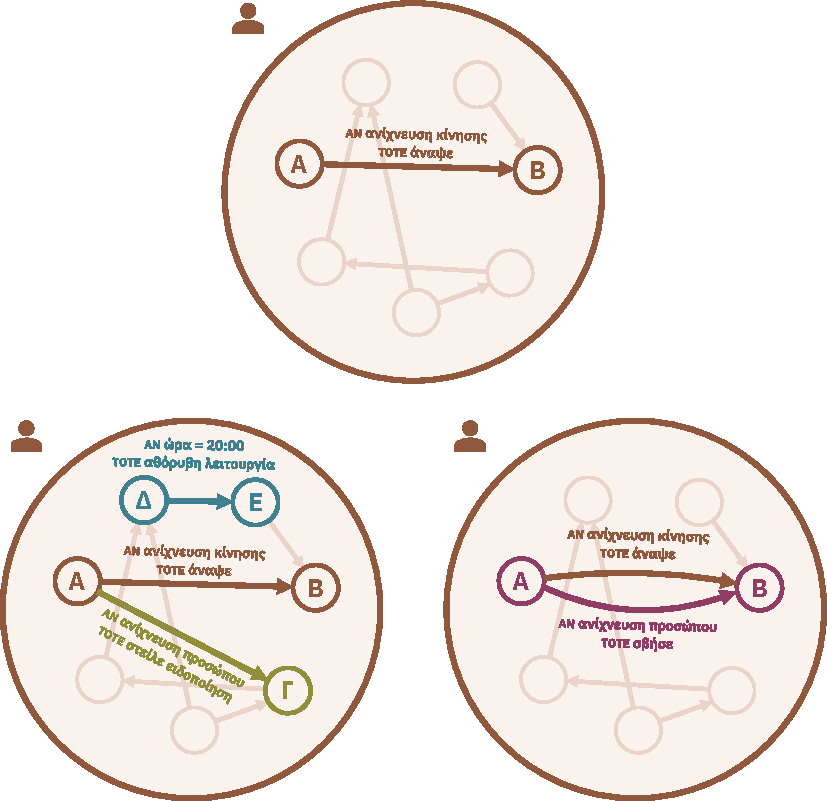
\includegraphics[width=\linewidth]{./assets/images/hard-negatives}
  \caption[Hard negatives]{Hard negatives: Πάνω φαίνεται η πραγματική (θετική) ακμή προς μελέτη (Α→Β). Κάτω αριστερά εικονίζονται δύο \textbf{απλά (soft) negatives}: το μπλε (Δ→Ε) έχει διαφορετικό source κόμβο (Δ αντί Α) και destination κόμβο (Ε αντί Β), ενώ το πράσινο (Α→Γ) έχει ίδιο source κόμβο (Α). Κάτω δεξιά εικονίζεται ένα \textbf{hard negative}: η νέα ακμή έχει \textbf{κοινό} τόσο τον source κόμβο (Α) όσο και τον destination (Β), με μόνη διαφορά σε σχέση με την θετική ακμή τον \textbf{τύπο} της ακμής («ανίχνευση προσώπου → σβήσε» αντί «ανίχνευση κίνησης → άναψε»). Πληροί έτσι τις δύο προϋποθέσεις των hard negatives: (α) έχει κοινό ζεύγος (src, dst) και διαφορετικό τύπο ακμής, και (β) δεν αποτελεί προϋπάρχουσα ακμή στον γράφο του χρήστη (ο αρχικός γράφος πάνω έχει μόνο μία ακμή από το Α στο Β, την υπό εξέταση).}
  \label{fig:hard-negatives}
\end{figure}

\begin{figure}[htbp]
  \centering
  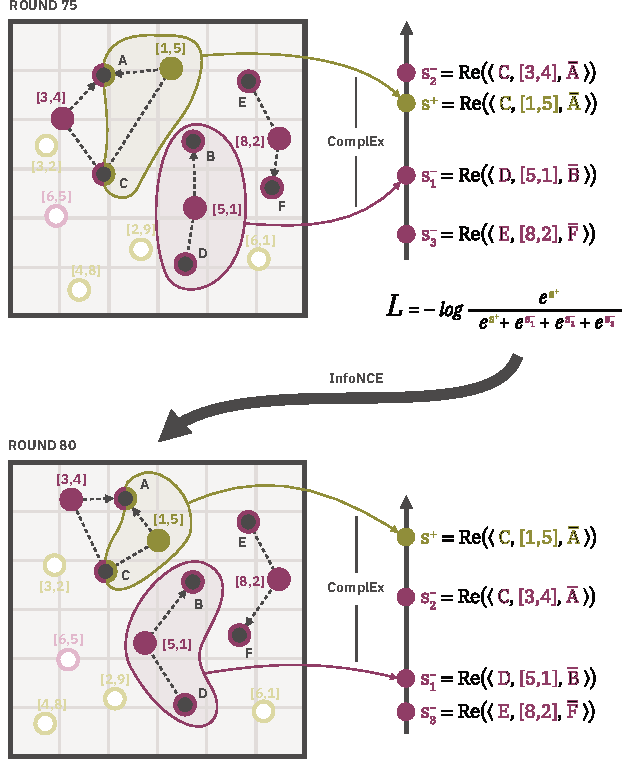
\includegraphics[width=0.8\linewidth]{./assets/images/infonce}
  \caption[InfoNCE loss]{InfoNCE loss σε δύο γύρους εκπαίδευσης: \textbf{Πάνω (γύρος 75):} το ComplEx μετατρέπει το positive edge \{C, [1,5], A\} σε ένα σκορ $s^+$, και τα negatives \{D, [5,1], B\}, \{C, [3,4], A\} και \{Ε, [8,2], F\} σε $s^-_1$, $s^-_2$ και $s^-_3$ αντίστοιχα, στον άξονα των πραγματικών. Η InfoNCE υπολογίζει το softmax τους (θετική στον αριθμητή, θετική συν άθροισμα αρνητικών στον παρονομαστή), πιέζοντας την θετική ακμή πάνω από όλες τις αρνητικές. \textbf{Κάτω (γύρος 80):} το CompGCN έχει αναμορφώσει τα embeddings ώστε η θετική να ξεπερνά πλέον και το hard negative $s^-_2$ που προηγουμένως προηγούνταν.}
  \label{fig:infonce}
\end{figure}

\begin{figure}[H]
  \centering
  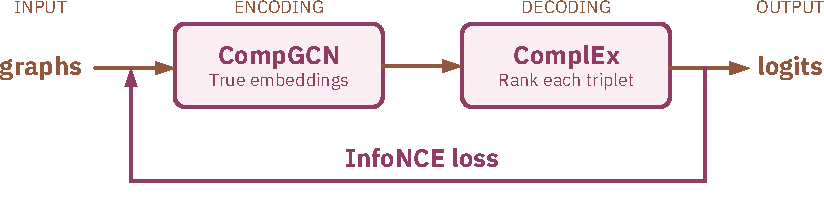
\includegraphics[width=0.95\linewidth]{./assets/images/v3-pipeline}
  \caption[Pipeline τρίτης έκδοσης]{Pipeline τρίτης έκδοσης: Το GraphSAGE αντικαθίσταται από το CompGCN για το encoding, ενώ το MLP αντικαθίσταται από το ComplEx για το decoding.}
  \label{fig:v3-pipeline}
\end{figure}

Ο συνδυασμός των τριών αυτών αλλαγών (CompGCN + ComplEx + InfoNCE με hard negatives) αποτελεί την τελική διαμόρφωση της υλοποίησης~(\autoref{fig:architecture}), η αποτελεσματικότητα της οποίας περιγράφεται αναλυτικά στην \autoref{sec:exp-results}.

\begin{figure}[htbp]
  \centering
  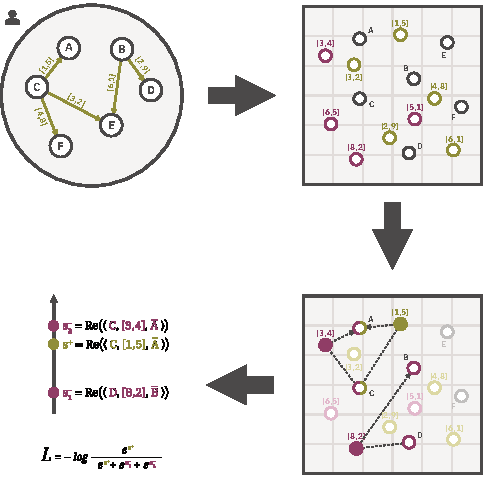
\includegraphics[width=\linewidth]{./assets/images/v3-detail-compact}
  \caption[Συνολική αρχιτεκτονική της τελικής υλοποίησης]{Συνολική αρχιτεκτονική της τελικής υλοποίησης (v3), από τον γράφο του χρήστη έως την απώλεια. Ο CompGCN encoder παράγει embeddings των κόμβων και των τύπων ακμών (πάνω), από τα οποία συναρμολογείται μια τριπλέτα $(h, r, t)$ (κάτω δεξιά). Στην συνέχεια ο ComplEx decoder μετατρέπει κάθε τριπλέτα σε ένα βαθμωτό score $s=\mathrm{Re}(\langle h, r, \bar t\rangle)$ (κάτω αριστερά). Η InfoNCE συγκρίνει το score της θετικής ακμής με εκείνα $K$ αρνητικών, και το gradient της αναμορφώνει τα embeddings.}
  \label{fig:architecture}
\end{figure}